\documentclass{ximera}

\newcommand{\dfn}{\textbf}
\renewcommand{\vec}[1]{{\overset{\boldsymbol{\rightharpoonup}}{\mathbf{#1}}}\hspace{0in}}
%% Simple horiz vectors
\renewcommand{\vector}[1]{\left\langle #1\right\rangle}
\newcommand{\arrowvec}[1]{{\overset{\rightharpoonup}{#1}}}
\newcommand{\R}{\mathbb{R}}
\newcommand{\transpose}{\intercal}
\newcommand{\ro}{\texttt{R}}%% row operation
\newcommand{\dotp}{\bullet}%% dot product

\usetikzlibrary{calc,bending}
\tikzset{>=stealth}


\usepackage{mdframed} % For framing content
%\usepackage{ifthen}   % For conditional statements

% Define the 'concept' environment with an optional header
\newenvironment{concept}[1][]{%
  \begin{mdframed}[linecolor=black, linewidth=2pt, innertopmargin=5pt, innerbottommargin=5pt, skipabove=12pt, skipbelow=12pt]%
    \noindent\large\textbf{#1}\normalsize%
}{%
  \end{mdframed}%
}











%% \colorlet{textColor}{black}
%% \colorlet{background}{white}
%% \colorlet{penColor}{blue!50!black} % Color of a curve in a plot
%% \colorlet{penColor2}{red!50!black}% Color of a curve in a plot
%% \colorlet{penColor3}{red!50!blue} % Color of a curve in a plot
%% \colorlet{penColor4}{green!50!black} % Color of a curve in a plot
%% \colorlet{penColor5}{orange!80!black} % Color of a curve in a plot
%% \colorlet{penColor6}{yellow!70!black} % Color of a curve in a plot
%% \colorlet{fill1}{penColor!20} % Color of fill in a plot
%% \colorlet{fill2}{penColor2!20} % Color of fill in a plot
%% \colorlet{fillp}{fill1} % Color of positive area
%% \colorlet{filln}{penColor2!20} % Color of negative area
%% \colorlet{fill3}{penColor3!20} % Fill
%% \colorlet{fill4}{penColor4!20} % Fill
%% \colorlet{fill5}{penColor5!20} % Fill
%% \colorlet{gridColor}{gray!50} % Color of grid in a plot


\author{Bart Snapp \and Parisa Fatheddin}
%%OpenAI. (2023). ChatGPT (Mar 14 version) [Large language model]. https://chat.openai.com/chat

\title{Vectors and scalars}


\begin{document}
\begin{abstract}
  A concrete introduction to vectors along with some examples of real world applications.
\end{abstract}
\maketitle


\begin{quote}
  Probably no other area of mathematics has been applied in such
  numerous and diverse contexts as the theory of matrices. In
  mechanics, electromagnetics, statistics, economics, operations
  research, the social sciences, and so on, the list of applications
  seems endless. By and large this is due to the utility of matrix
  structure and methodology in conceptualizing sometimes complicated
  relationships and in the orderly processing of otherwise tedious
  algebraic calculations and numerical manipulations.



  \hfill ---\link[J.\ Cochran]{https://www.amazon.com/Applied-Mathematics-Principles-Applications-Probability/dp/0534980260}
\end{quote}


\section{Vectors and scalars}

In mathematics, we study (among other things) numbers. In many cases,
these numbers represent real-world data. Sometimes it ``makes sense''
to add data and sometimes it doesn't.
\begin{concept}[When it does NOT make sense to add data]
\begin{description}
\item[Personal Identification Numbers] Summing things like social
  security numbers, phone numbers, or zip codes doesn't provide
  meaningful information.
\item[Temperatures] While you can mathematically add temperatures
  together, doing so usually doesn't provide useful information.
\item[Time] Adding specific points in time, like dates or hours of the
  day, usually doesn't yield meaningful results.
\item[Geographic Coordinates] Adding the latitude and longitude of two
  locations doesn't give you a location that has any real-world
  significance.
\end{description}
\end{concept}
For some of the categories above, the \textit{average} can be
meaningful or perhaps if each quantity is thought of as `displacement'
or `duration,' summing might be meaningful. However, without
additional (pun intended!) stipulations, summing the types of
quantities above is not meaningful. On the other hand, there are lots
of times that it makes sense to add data:

\begin{concept}[When it makes sense to add data]
\begin{description}
\item[Population Counts] Adding the populations of different regions,
  cities, or countries to find the total population of a larger
  area. Answers to questions like these help us understand our
  society and are important to many people.
\item[Financial Transactions] Summing daily sales to find total
  monthly sales, or adding up all expenses to find total costs. These
  are real numbers that represent actual amounts of money, and their
  total gives meaningful information about financial status or
  performance.
%% \item[Time Spent on Tasks] Adding the duration of time spent on
%%   various activities on day gives a total time spent. We all have busy
%%   lives, and time is a very precious commodity. Hence, it is good to
%%   understand how we spend our time.
\item[RGB Color Space] Colors on digital screens are often represented
  as vectors in the \link[RGB color space]{https://en.wikipedia.org/wiki/RGB_color_model}. Here three numerical components
  correspond to the intensity of red, green, and blue light, with $0$
  representing no intensity, black can be represented by $(0,0,0)$,
  and $255$ represents maximum intensity, white can be represented by
  $(255,255,255)$.  Adding the values for different pixels changes the
  brightness of each individual component.
\item[Navigation] Aircraft navigate by knowing the direction and speed \textcolor{blue}{at which}
  they are traveling. When interpreted correctly, we add the
  speed and direction of many different ``course changes'' to
  find the ultimate position of the aircraft.
\end{description}
\end{concept}
Often when it makes sense to \textit{add} quantities, it makes sense
to \textit{scale} them as well. For example with population, you could
ask for the population of a city with $3$ times the population, or
half the population. In a similar way, \textit{scaling} makes sense
for all the examples above where it \textcolor{blue}{makes} sense to
add data. Regular old numbers used to scale vectors are called
\textit{scalars}.


\begin{definition}
  We say data is represented by \dfn{vectors} $\vec{v}$ and $\vec{w}$
  if
  \[
  \vec{v}+\vec{w}
  \]
  is also a vector, encoding `meaningful' data in the same way that
  $\vec{v}$ and $\vec{w}$ do, and for all \textbf{scalars} $s$, where
  $s$ is usually a real number,
  \[
  s(\vec{v} + \vec{w}) = s\vec{v}+ s\vec{w}.
  \]
  again represents `meaningful' data in the same way that $\vec{v}$
  and $\vec{w}$ do.
\end{definition}
These informal definitions of vectors and scalars in fact contain the
\textit{essence} of the concept of a \textit{vector space}. If this
seems too abstract, let's give some very concrete examples, based on
the examples above. However, before we start, we need to give some
notation for vectors.

\begin{concept}[Ways data can be stored as a vector]
\begin{description}
\item[Ordered tuple] An ordered pair is just a pair of numbers
  $(a,b)$ delineated by parenthesis with the entries separated by a
  comma. It's called ``ordered'' because $(a,b) \ne (b,a)$. An \textit{ordered
  tuple} is just a list of an arbitrary, but fixed, number of elements
  that is ordered like an ordered pair. As an example, we could
  represent the \link[demographic information]{https://worldpopulationreview.com/states/states-by-race} for Ohio as an vector
  represented by an ordered tuple:
  \[
  \vec{p}_{\texttt{OH}} = (\underset{\text{White}}{9394878},\underset{\text{Black}}{1442655},\underset{\text{American Indian}}{20442},\underset{\text{Asian}}{268527},\underset{\text{Hawaiian}}{3907},\underset{\text{Other}}{544866})
  \]
\item[Row vector] A row vector is a lot like an ordered tuple, except
  we do not use a comma to separate entries. Instead, we separate them
  by some space.  Suppose a bookstore sells a variety of books in a
  month, say $141$ Science Fiction, $304$ Fantasy, $249$ Mystery,
  $199$ Romance, $251$ \textcolor{blue}{History}.  We can express this
  data as a row vector:
  \[
  \vec{s} = \begin{pmatrix}141 & 304 & 249 & 199 & 251 \end{pmatrix}
  \]
  \item[\textcolor{blue}{Column vector}] A column vector is just like a row vector,
  except is it written vertically:
  \[
  \vec{p} = \begin{pmatrix}
    159\\  226 \\ 191\end{pmatrix}
    \qquad
    \begin{array}{l}
    \text{Red}\\
    \text{Green}\\
    \text{Blue}
    \end{array}
  \]
  Above, we suppose that $\vec{p}$ represents the color that
  represents the color \textit{Sea Foam Green}.
%% \item[As a column vector] A column vector is just like a row vector,
%%   except is it written vertically:
%%   \[
%%   \vec{w}_{\texttt{TR}} = \begin{pmatrix}
%%     0.5\\ 4 \\ 0 \\ 1\end{pmatrix}
%%     \qquad
%%     \begin{array}{l}
%%     \text{Emails}\\
%%     \text{Classes}\\
%%     \text{Projects}\\
%%     \text{Exercising}
%%   \end{array}
%%   \]
%%   Above, we could suppose that $\vec{w}_{\texttt{TR}}$ represents the
%%   fact that on Tuesdays and Thursdays, someone spends $0.5$ hours on
%%   emails, $4$ hours in class, $0$ hours on projects, and $1$ hour
%%   exercising.
\end{description}
\end{concept}

Of course, since mathematics is a human endeavor you will find
variations on the notations above. As a common example, some folks use
different brackets like these
\[
\langle a, b, c\rangle, \quad \begin{bmatrix} a & b & c \end{bmatrix}, \quad \text{or}\quad
\begin{bmatrix}
  a\\
  b\\
  c
\end{bmatrix}
\]
for an ordered-tuple vectors, row vectors, and column vectors. Ordered
tuples and row vectors are easy to write in-line (in a sentence),
because they are horizontal. On the other hand, column vectors take up
less horizontal space and are more convenient when you have vectors
with many entries.


\begin{definition}
  To switch a row vector into a column vector and vice versa, we use
  the \dfn{transpose} operation, referred to as the transpose of the
  vector,
  \[
  \begin{pmatrix} 1 &  2 & 3 \end{pmatrix}^\transpose =
  \begin{pmatrix} 1 \\ 2 \\ 3 \end{pmatrix}
  \quad\text{and}\quad
  \begin{pmatrix} 1 \\ 2 \\ 3 \end{pmatrix}^\transpose =
  \begin{pmatrix} 1 &  2 & 3 \end{pmatrix}
  \]
\end{definition}


\begin{question}
  Consider $\vec{s} = \begin{pmatrix}141 & 304 & 249 & 199 & 251 \end{pmatrix}$. Compute $\vec{s}^\transpose$.
  \begin{prompt}
  \[
  \vec{s}^\transpose  = \begin{pmatrix}\answer{141} \\ \answer{304} \\ \answer{249} \\ \answer{199} \\ \answer{251} \end{pmatrix}
  \]
  \end{prompt}
\end{question}

Once we have data represented as vectors encoded as ordered tuples,
row vectors, or column vectors, we can describe some general
information about the vectors. In particular, we can think about their
\textit{dimension} and their \textit{components}.

\begin{definition}
The \dfn{dimension} of a vector is the number of entries. Each
individual entry of a vector is called a \dfn{component}.
\end{definition}

\begin{question}
  What is the dimension of the vector $\vec{p}_{\texttt{OH}}$?
  \begin{prompt}
  \[
  \text{Dimension} = \answer{6}
  \]
  \end{prompt}
\end{question}


When we express vectors as ordered tuples, row vectors, or column
vectors we add them in a componentwise fashion.
\begin{align*}
  (1,2,3) + (4,5,6) &= (5,7,9)\\
  \begin{pmatrix} 1 & 2 & 3   \end{pmatrix} + \begin{pmatrix} 4 & 5 & 6   \end{pmatrix}& = \begin{pmatrix} 1+4 & 2+5 & 3+6   \end{pmatrix}&= \begin{pmatrix} 5 & 7 & 9   \end{pmatrix}\\
  \begin{pmatrix} 1\\ 2\\ 3   \end{pmatrix} + \begin{pmatrix} 4\\ 5\\ 6   \end{pmatrix} &= \begin{pmatrix} 5\\ 7\\ 9   \end{pmatrix}
\end{align*}

We can also multiply vectors by a \dfn{scalar} (a number), by
multiplying each component by the scalar.
\begin{align*}
  5\cdot   (1,2,3) &= (5,10,15)\\
  5\cdot \begin{pmatrix} 1 & 2 & 3   \end{pmatrix}  &= \begin{pmatrix} 5 & 10 & 15   \end{pmatrix}\\
  5\cdot  \begin{pmatrix} 1\\ 2\\ 3   \end{pmatrix} &= \begin{pmatrix} 5\\ 10\\ 15   \end{pmatrix}
\end{align*}
Now that we know the basics, onto the examples!

\begin{example}[Population Counts] %https://worldpopulationreview.com/states/states-by-race
  The Midwest of the United States consists of $12$ states. We can
  express the $2023$
  \link[demographics]{https://worldpopulationreview.com/states/states-by-race}
  of each state as a vector represented by an ordered tuple. The
  ordered tuple for Ohio looks like:
  \[
  \vec{p}_{\texttt{OH}} = (\underset{\text{White}}{9394878},\underset{African American}{1442655},\underset{\text{American Indian}}{20442},\underset{\text{Asian}}{268527},\underset{\text{Hawaiian}}{3907},\underset{\text{Other}}{544866}).
  \]
  The ordered tuples for each state in the Midwest looks like:
\begin{align*}
  \vec{p}_{\texttt{IA}} &= (2806418,117035,10538,79296,3941,132783)\\
  \vec{p}_{\texttt{IL}} &= (8874067,1796660,33972,709567,5196,1296702)\\
  \vec{p}_{\texttt{IN}} &= (5510354,631923,14030,158705,2205,379676)\\
  \vec{p}_{\texttt{KA}} &= (2416165,165837,22278,87093,2344,218902)\\
  \vec{p}_{\texttt{MI}} &= (7735902,1360149,50035,316844,3117,507860)\\
  \vec{p}_{\texttt{MN}} &= (4572149,359817,54558,275242,2201,336199)\\
  \vec{p}_{\texttt{MO}} &= (4978046,698043,24274,123810,8887,291100)\\
  \vec{p}_{\texttt{ND}} &= (651470,23959,39165,11979,1004,32817)\\
  \vec{p}_{\texttt{NE}} &= (1641256,91896,16875,47944,1235,124620)\\
  \vec{p}_{\texttt{OH}} &= (9394878,1442655,20442,268527,3907,544866)\\
  \vec{p}_{\texttt{SD}} &= (735228,18836,74975,12413,544,37340)\\
  \vec{p}_{\texttt{WI}} &= (4895065,367889,48674,163396,2672,329279)
\end{align*}
\begin{enumerate}
\item What are the combined demographics of the states Michigan, Ohio,
  and Indiana?
\item Suppose that the annual percentage growth rate of Ohio is
  currently $0.1\%$. Assuming this is even across all demographics,
  what might the population data look like for Ohio in $2025$?
\end{enumerate}
\begin{explanation}
  We'll use the properties of vectors to solve this problem.
  \begin{enumerate}
  \item To find the combined demographics of Michigan, Ohio, and
    Indiana we compute
    \[
    \vec{p}_{\texttt{MI}} + \vec{p}_{\texttt{OH}} + \vec{p}_{\texttt{IN}} = \left(\answer[given]{22641134},\answer[given]{3434727},\answer[given]{84507},744076,9229,1432402\right)
    \]
  \item To find the population growth of each demographic, we use the scalar, $1.001$ to find:
    \[
    1.001 \vec{p}_{\texttt{OH}} =\left(\answer[given]{9404273},\answer[given]{1444098},\answer[given]{20462},268796,3911,545411 \right)
    \]
  \end{enumerate}
\end{explanation}
\end{example}



\begin{example}[Financial Transactions]
  A bookstore sells a variety of books. We'll express the number of
  each type of book sold in one month as a row vector
  \[
  \vec{s} = \begin{pmatrix}141 & 304 & 249 & 199 & 251 \end{pmatrix}
  \]
  with the entries representing the categories: Science Fiction,
  Fantasy, Mystery, Romance, History in that order.  If each book
  costs the bookstore $6$ dollars from the wholesaler, and each book sells
  for $9$ dollars, what is the profit for each category?
  \begin{explanation}
    Using the properties of vectors, we wish to compute:
    \[
    9\vec{s}-6\vec{s} = \begin{pmatrix} \answer[given]{423} & \answer[given]{912} & \answer[given]{747} & 597 & 753 \end{pmatrix}
    \]
  \end{explanation}
\end{example}


\begin{example}[RGB Color Space]
  The \textit{MOOCulus Lighting Company} has designed an LED table
  lamp whose shades vary linearly, at a constant rate, through six
  colors ($3$ primary and $3$ secondary) of the RGB color space in
  this order:
    \[
    \underset{\text{red}}{\begin{pmatrix}255\\0\\0\end{pmatrix}},
    \underset{\text{yellow}}{\begin{pmatrix}255\\255\\0\end{pmatrix}},
    \underset{\text{green}}{\begin{pmatrix}0\\255\\0\end{pmatrix}},
    \underset{\text{cyan}}{\begin{pmatrix}0\\255\\255\end{pmatrix}},
    \underset{\text{blue}}{\begin{pmatrix}0\\0\\255\end{pmatrix}},
    \underset{\text{magenta}}{\begin{pmatrix}255\\0\\255\end{pmatrix}}, 
    \]
  If the lamp is turned on, it initally shows, red, then this fades to
  yellow after one minute, then fades green after a minute more, and
  so on. After $6$ minutes it is back to red. Color $\vec{c}_1$ fades
  to $\vec{c}_2$ like the vector function $\vec{f}(t)$
  \[
  \vec{f}(t) = \vec{c}_1+ t(\vec{c}_2 -\vec{c}_1)
  \]
  as $t$ runs from $0$ to $1$. Note $\vec{f}(0) = \vec{c}_1$ and
  $\vec{f}(1) = \vec{c}_2$.  What RGB color is the lamp showing at $4$
  minutes and $40$ seconds?
  \begin{explanation}
    At $4$ minutes and $40$ seconds, our lamp is showing some color
    between blue and magenta. Let
    \[
    \vec{c}_1 = \begin{pmatrix}0\\0\\255\end{pmatrix} \quad\text{and}\quad
      \vec{c}_2 = \begin{pmatrix}255\\0\\255\end{pmatrix} 
    \]
    Since $40$ seconds is $2/3$ of a minute, we write
    \begin{align*}
      \vec{f}(2/3) &= \vec{c}_{1}+ \left(\answer[given]{2/3}\right)(\vec{c}_2 -\vec{c}_1) \\
      &= \begin{pmatrix}0\\0\\255\end{pmatrix}+ \left(\answer[given]{2/3}\right)\left(\begin{pmatrix}255\\0\\255\end{pmatrix}  -  \begin{pmatrix}0\\0\\255\end{pmatrix}\right) \\
      &=\begin{pmatrix}0\\0\\255\end{pmatrix}+ \left(\answer[given]{2/3}\right)\begin{pmatrix}255\\0\\0\end{pmatrix} \\
              &=\begin{pmatrix}0\\0\\255\end{pmatrix}+ \left(\answer[given]{2/3}\right)\begin{pmatrix}255\\0\\0\end{pmatrix}\\
                &=\begin{pmatrix}170\\0\\255\end{pmatrix}
    \end{align*}
    Here is this color:
  \begin{center}
    \colorbox[rgb]{0.667, 0, 1}{%(170,0, 255)
      \parbox{1cm}{\rule{0pt}{1cm}}}
  \end{center}
  \end{explanation}
\end{example}





%% \begin{example}[Time Spent on Tasks]
%%   On Mondays, Wednesdays, and Fridays, suppose you spend you spend $1$
%%   hour on emails, $2$ hours in class, and $3$ hours working on
%%   projects. On Tuesdays and Thursdays, you spend $1/2$ hour on emails,
%%   $4$ hours in class, and $1$ hour exercising. We can express each day
%%   as a column vector:
%%   \[
%%   \vec{w}_{\texttt{MWF}} =
%%   \begin{pmatrix}
%%     1 \\
%%     2 \\
%%     3 \\
%%     0
%%   \end{pmatrix}
%%   \qquad
%%   \vec{w}_{\texttt{TR}} =
%%   \begin{pmatrix}
%%     0.5\\
%%     4\\
%%     0\\
%%     1
%%   \end{pmatrix} \qquad
%%   \begin{array}{l}
%%     \text{Emails}\\
%%     \text{Classes}\\
%%     \text{Projects}\\
%%     \text{Exercising}
%%   \end{array}
%%   \]
%%   How much time is spent on emails, classes, projects, and exercising
%%   per work week?
%%   \begin{explanation}
%%     Here we simply compute:
%%     \[
%%     3 \vec{w}_{\texttt{MWF}} + 2  \vec{w}_{\texttt{TR}}  =
%%     \]
%%   \end{explanation}
%% \end{example}







\begin{example}[Navigation]
  Airplanes can use true bearings for navigation. Here's the idea: the
  direction given by degrees from North is found by:

\begin{center}
\upshape
% Define a few constants for easy configuration
\def\radius{2cm}
\def\onedegrad{1.8cm}
\def\fivedegrad{1.75cm}
\def\tendegrad{1.7cm}
\def\labelrad{1.6cm}

\begin{tikzpicture}[scale=1.3] %% https://texample.net/tikz/examples/degree-wheel/
  \draw[ultra thick] (0,0) circle (\radius);
  % labels and longer lines at every 10 degrees
  \node at (0,.65*\radius) {\bf N};
  \node at (0,-.65*\radius) {\bf S};
  \node at (-.65*\radius,0) {\bf W};
  \node at (.65*\radius,0) {\bf E};
  \foreach \x in {0,10,...,350}
  {
    \node[scale=.5, rotate=\x*-1] at (360-\x+90:\labelrad) {\x};
    \draw[thick] (\x:\tendegrad) -- (\x:\radius);
  };

  % lines at every 5 degrees
  \foreach \x in {0,5,...,355}  \draw (\x:\fivedegrad) -- (\x:\radius);

\end{tikzpicture}
\end{center}

So traveling North would be a (true) bearing of $0^\circ$, while
traveling West would be a bearing of $270^\circ$.
\link[knots]{https://en.wikipedia.org/wiki/Knot_(unit)}.
\begin{enumerate}
\item Suppose a plane starts at $(0,0)$ and its destination is reached
  by following true bearing $280^\circ$ for $3$ hours at $125$ knots.
  What are the coordinates of the plane's destination?
\item Suppose the plane travels at $125$ by true bearing of $280^\circ$ for $3$ hours then the wind starts blowing and make it travel at $35$ knots in the true
  bearing of $110^\circ$ for another $3$ hours. What are the coordinates of
  the plane after these times?
%% \item What course and speed should the pilot set to arrive at the
%%   destination on-time?
\end{enumerate}

\begin{explanation}
While it makes sense (separately) to add speeds and angles, we cannot
directly make a vector from this information because there is no
obvious way to ``add'' ordered tuples of speed and angle. However, we
can convert a true bearing of $\beta$ along with a speed $v$ to
cartesian coordinates by writing:
\[
\begin{pmatrix}v\cdot \sin(\beta)\\ v \cdot \cos(\beta)\end{pmatrix}
\]
Armed with this, we are ready to solve the problem.
\begin{enumerate}
\item  Converting the planes bearing and speed to a vector in cartesian
  coordinates, we have
  \[
  \vec{p} = \begin{pmatrix}125\cdot \sin(280^\circ)\\ 125 \cdot \cos(280^\circ)\end{pmatrix}
  \]
  Here is a schematic drawing of what is happening:

  \begin{center}
    %% A schematic diagram showing a vector at a 330 degree angle with a
    %% vertical line, made in a clockwise fashion. The vectors' length is labeled 125
    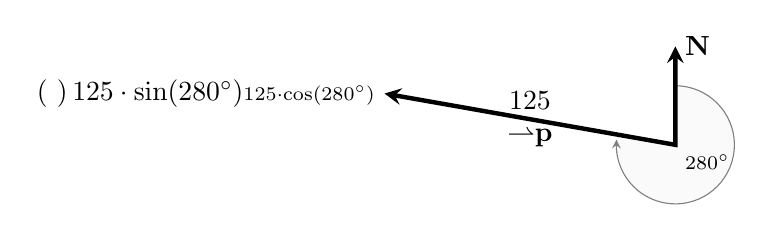
\begin{tikzpicture}[scale=2.5]
      \filldraw[fill=black!2!white,draw=none]
      (0,0) -- (0mm,3mm) arc (90:-190:3mm) -- (0,0);

      \draw[draw=white!50!black,->]
      (0mm,3mm) arc (90:-185:3mm);

      \draw[<->,ultra thick] ({1.5*sin(280)},{1.5*cos(280)}) -- (0,0) -- (0,.5);

      \node[below right] at (0,0) {$\scriptstyle 280^\circ$};
      \node[right] at (0,.5) {\bf N};
      \node[above]  at ({.75*sin(280)},{.75*cos(280)}) {$125$};
      \node[below]  at ({.75*sin(280)},{.75*cos(280)}) {$\vec{p}$};
      \node[left] at ({1.5*sin(280)},{1.5*cos(280)}) {$\begin{pmatrix}\scriptstyle 125\cdot \sin(280^\circ)\\ \scriptstyle 125 \cdot \cos(280^\circ)\end{pmatrix}$};
    \end{tikzpicture}
  \end{center}



To find the coordinates of the plane after it has traveled for $3$
hours, we use $3$ as a scalar to write (round to two decimal places).
\begin{align*}
  3\vec{p} &= \begin{pmatrix}\answer[given]{375}\cdot \sin(280^\circ)\\ \answer[given]{375} \cdot \cos(280^\circ)\end{pmatrix}\\
  &= \begin{pmatrix}\answer[given]{-369.30}\\ \answer[given]{65.12} \end{pmatrix}\\
\end{align*}
\item Now supposing that the wind \textcolor{blue}{is} blowing at $35$ knots in the true
  bearing of $110^\circ$, we have something like this:
  \begin{center}
    %% A schematic diagram showing a vector at a 330 degree angle with a
    %% vertical line, made in a clockwise fashion. The vectors' length is labeled 125
    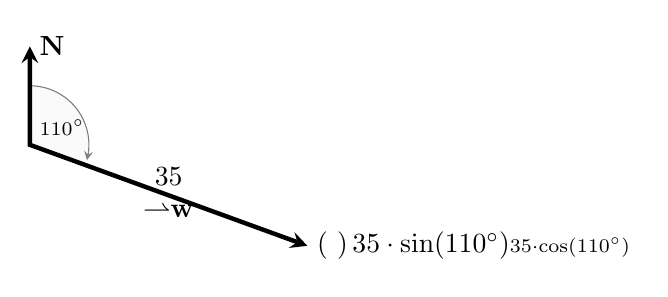
\begin{tikzpicture}[scale=2.5]
      \filldraw[fill=black!2!white,draw=none]
      (0,0) -- (0mm,3mm) arc (90:-20:3mm) -- (0,0);

      \draw[draw=white!50!black,->]
      (0mm,3mm) arc (90:-15:3mm);

      \draw[<->,ultra thick] ({1.5*sin(110)},{1.5*cos(110)}) -- (0,0) -- (0,.5);

      \node[above right] at (0,0) {$\scriptstyle 110^\circ$};
      \node[right] at (0,.5) {\bf N};
      \node[above]  at ({.75*sin(110)},{.75*cos(110)}) {$35$};
      \node[below]  at ({.75*sin(110)},{.75*cos(110)}) {$\vec w$};
      \node[right] at ({1.5*sin(110)},{1.5*cos(110)}) {$\begin{pmatrix}\scriptstyle 35\cdot \sin(110^\circ)\\ \scriptstyle 35 \cdot \cos(110^\circ)\end{pmatrix}$};

    \end{tikzpicture}
  \end{center}
  So now we can solve our problem by computing (round to two decimal places):
  \[
  3\vec{p} + 3 \vec{w} = \textcolor{blue}{\begin{pmatrix} \answer[given]{-369.3}\\ \answer[given]{65.12} \end{pmatrix} + \begin{pmatrix} \answer[given]{32.89} \\
  \answer[given]{-11.97} \end{pmatrix} = \begin{pmatrix} \answer[given]{-336.41} \\ \answer[given]{53.15}\end{pmatrix}}
  \]
\end{enumerate}
\end{explanation}
\end{example}

\end{document} 
